\documentclass[8pt]{beamer}
\usepackage{listings}
\usetheme{Darmstadt}
\setbeamertemplate{footline}[frame number]
\usepackage{graphics}
\usepackage{pgf, tikz}
\usepackage{fancybox}
\usepackage{amssymb}
\usepackage{subcaption}
\usetikzlibrary{arrows, automata,calc}
\usetikzlibrary{er,positioning}
\title{Using Reachability Properties of Logic Program for Revising Biological Models}
\author{Xinwei Chai, Tony Ribeiro, Morgan Magnin, Olivier Roux, Katsumi Inoue}
\date{September 4, 2018}
\input{macros}
\input{macros-ph}
\input{macros-abstr}
\input{tikzstyles2}
\tikzstyle{block} = [rectangle, draw, fill=blue!20, 
    text width=6em, text centered, rounded corners, minimum height=4em]
    \tikzstyle{line} = [draw, -latex']

\begin{document}
\maketitle


\begin{frame}{Outline}
\begin{columns}
\begin{column}{0.7\textwidth}
    \begin{figure}
       \centering
       \includegraphics[height=0.7\paperheight]{systems_biology.png}
   \end{figure}
\end{column}
\begin{column}{0.3\textwidth}
%More precisely:
    \only<2>{
    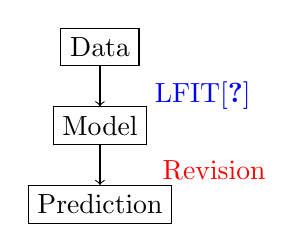
\begin{tikzpicture}
        \node [draw](data) {Data};
        \node [draw,below of = data] (model) {Model};
        \draw[->] (data) -- (model);
        \node [draw,below of = model] (pred) {Prediction};
        \draw[->] (model) -- (pred);
        \node [below right = 0.1cm of data] (LFIT){\textcolor{blue}{LFIT\cite{ribeiro2013bdd}}};
        \node [below right = 0.1cm of model] (Revision){\textcolor{red}{Revision}};
    \end{tikzpicture}
    }
\end{column}
\end{columns}
\end{frame}
\begin{frame}{Process Scheme}
\begin{figure}
    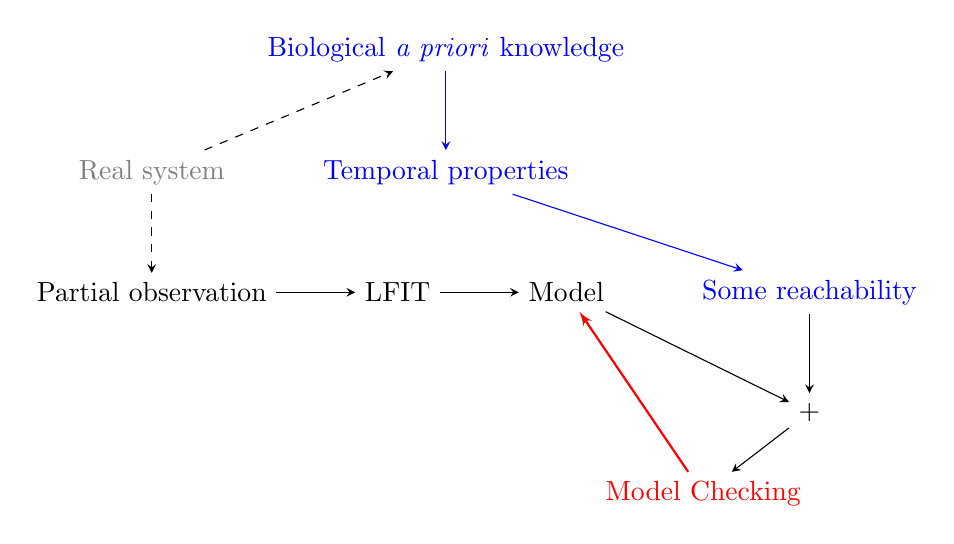
\begin{tikzpicture}[line,>=stealth]
        \node [color=gray] (1) {Real system};
        \node [color=blue,right = of 1] (2) {Temporal properties};
        \node [below = of 1] (3) {Partial observation};
        \node [right = of 3] (4) {LFIT};
        \node [right = of 4] (8) {Model};
        \draw [->] (4) -- (8);
        \node [color=blue,right = of 8] (5) {Some reachability};
        \node [color = red, below left = 2cm and -1.5cm of 5] (7) {Model Checking};
        \node [color=blue,above = of 2] (6) {Biological \textit{a priori} knowledge};
        \draw [dashed,->] (1) -- (6);
        \draw [color=blue,->] (2) -- (5);
        \draw [dashed,->] (1) -- (3);
        \draw [->] (3) -- (4);
        %\draw [->] (8) -- (5);
        \draw [color=blue, ->] (6) -- (2);
        \node [below = of 5] (9) {$+$};
        \draw [->] (8) --(9);
        \draw [->] (5) --(9);
        \draw [->] (9) --(7);
        \draw[thick, color=red] (7)--(8);
    \end{tikzpicture}
\end{figure}
    
\end{frame}

%\begin{frame}{Table of Contents}
%    \tableofcontents
%\end{frame}

\section{Modeling framework}% \& static analysis}
\begin{frame}{Modelings}
\begin{columns}

\begin{column}{.45\textwidth}
\centering
Boolean Network

\vspace{0.5cm}

$a(t+1)= \lnot b(t)$

$b(t+1)=a(t)$




\end{column}
\begin{column}{.1\textwidth}
\centering
$\Longleftrightarrow$
\end{column}
\begin{column}{.45\textwidth}
\centering
Logic Program

\vspace{0.5cm}

$a(t+1)\gets \lnot b(t)$

$b(t+1)\gets a(t)$


\end{column}
\end{columns}
%\vspace{0.5cm}
% Asynchronous Automata Network (AAN):
\begin{figure}
    \centering
    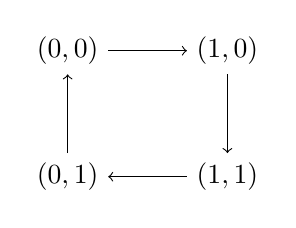
\begin{tikzpicture}
\node (00) {$(0,0)$};
\node [below = 1cm of 00] (01) {$(0,1)$};
\node [right = 1cm of 01] (11) {$(1,1)$};
\node [right = 1cm of 00] (10) {$(1,0)$};
\draw[->] (00) -- (10);
\draw[->] (10) -- (11);
\draw[->] (11) -- (01);
\draw[->] (01) -- (00);

\end{tikzpicture}

\end{figure}
\end{frame}


\section{Reachability analysis}
\begin{frame}{Reachability problem}
\begin{columns}
	\begin{column}{.5\textwidth}
	\centering
	\begin{figure}
    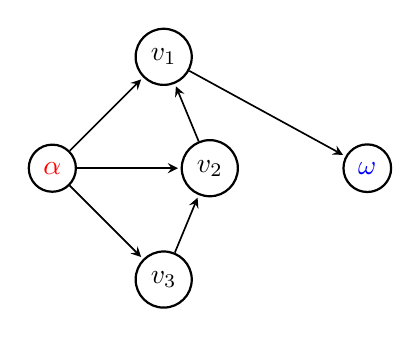
\begin{tikzpicture}[
            > = stealth, % arrow head style
            shorten > = 1pt, % don't touch arrow head to node
            auto,
            node distance = 2cm, % distance between nodes
            semithick % line style
        ]

        \tikzstyle{every state}=[
            draw = black,
            thick,
            fill = white,
            minimum size = 4mm
        ]

        \node[state] (s) {\textcolor{red}{$\alpha$}};
        \node[state] (v1) [above right of=s] {$v_1$};
        \node[state] (v2) [right of=s] {$v_2$};
        \node[state] (v3) [below right of=s] {$v_3$};
        \node[state] (t) [right of=v2] {\textcolor{blue}{$\omega$}};

        \draw[->] (s) -- (v1);
        \draw[->] (s) -- (v2);
        \draw[->] (s) -- (v3);
        \draw[->] (v2) -- (v1);
        \draw[->] (v3) -- (v2);
        \draw[->] (v1) -- (t);

    \end{tikzpicture}
    \end{figure}
    
    \end{column}
    \begin{column}{.5\textwidth}
    Given a BN, from initial state $\alpha$, does there exist a transition sequence that reaches the target state $\omega$?

    \vspace{0.25cm}
    
{\centering $\Updownarrow$

}
    
    \vspace{0.25cm}
   
   
    Given a state transition graph, from initial state $\alpha$, does there exist a pathway towards the target state $\omega$?
    \end{column}
\end{columns}

\vspace{0.1cm}

%The size of state transition graph is of $O(val^n)$, with $val$ the number of possible values of automata and $n$ the number of automata

\vspace{0.1cm}

Reachability of global states \fbox{$\mathbf{EF}(a_i,b_j,\ldots)$} $\to$ computationally difficult 

$\implies$ Reachability of local states \fbox{$\mathbf{EF}a_i$}

\end{frame}



\begin{frame}{Difficulties and solution}
\begin{itemize}
\item State space grows exponentially with the number of automata
\item Traditional model checkers e.g. Mole\footnote{\url{http://www.lsv.fr/~schwoon/tools/mole}} and NuSMV\footnote{\url{http://nusmv.fbk.eu}} fail

global search $\to$ time out and/or out of memory
\item \textbf{Static analysis}: avoid global search, at the cost of precision
\end{itemize}
$\to$ A balance between time-space performance and conclusiveness
\vspace{0.25cm}
\begin{itemize}
    \item Paulev\'e \textit{et al.} introduced LCG (Local Causality Graph) \cite{folschette2015,pauleve2012} for static analysis
    \item Implementation: Pint
\end{itemize}

\begin{itemize}
    \item Efficient (beats many traditional model checkers) \textbf{but}
    \item Usually not conclusive when the sparsity of the biological network increases
\end{itemize}
\end{frame}

\begin{frame}{Local Causality Graph (LCG)}
Start with target state $\omega\to$ Find transitions reaching $\omega\to$ Find new target states to fire those transitions $\to\cdots$ Recursion $\cdots\to$ End with initial state $\alpha$

\begin{itemize}
\item Goal-oriented structure 
\item Formed by recursive updates
%starting with desired final state, for each update, link the states with their associated transitions if they are not at initial state. Update ends when the graph becomes saturated.
\item Avoid global search in state transition graphs
\end{itemize}

\end{frame}


%\begin{frame}{Algorithm for Reachability}
%    \begin{itemize}
%    \item Input: An Automata Network $A$ and 2 partial states $init, target$ 
%    \item Output: \textbf{UNREACHABLE, REACHABLE, INCONCLUSIVE}
%\end{itemize}
%\begin{enumerate}
%    \item Construct the LCG $\ell=LCG(A,target)$
%    \item Check pseudo-reachability, can return \textbf{UNREACHABLE}
%    \item Clean all cycles and prune $\ell$
%    \item \textcolor{blue}{
%     Try at most $k$ times}
%    \begin{itemize}
%    \item \textcolor{blue}{$\ell'\gets \ell$}
%    \item \textcolor{blue}{ Transform randomly each OR gate $O$ of $\ell'$ into simple gate}
%    \item\textcolor{blue}{ Generate all trajectories $t$ to reach $target$ in $\ell$ using ASP}
%    \begin{itemize}
%        \item\textcolor{blue}{ If a valid $t$ is found, return \textbf{REACHABLE}}
%    \end{itemize}
%    \end{itemize}
%    \item\textcolor{blue}{ return \textbf{INCONCLUSIVE}}
%\end{enumerate}
%\end{frame}


\begin{frame}{Example of LCG}

Initial state $\alpha=\langle a_0,b_1,c_0,d_0,e_0\rangle$, target state $\omega=a_1$
\vspace{0.5cm}


Rules: \textcolor<3,5,6>{red}{$a_1\gets \{b_1, c_1\}$}, 
\textcolor<2,4>{red}{$a_1\gets e_1$},

\textcolor<7>{red}{$b_1\gets d_0$}, 
\textcolor<8>{red}{$c_1\gets d_1$}, 
\textcolor<10>{red}{$d_1\gets b_1$}

\vspace{0.5cm}

\begin{figure}

\input{LCGexampleAN}

\end{figure}
Small circles stand for transition nodes, squares for state nodes

\only<6>{$r'(a_1)=r'(e_1)\lor (r'(b_1)\land r'(c_1)$)}
\only<7>{$r'(a_1)=r'(d_0)\land r'(c_1)$}
\only<8>{$r'(a_1)=r'(d_0)\land r'(d_1)$}
\only<9>{$r'(a_1)=r'(d_1)$}
\only<10>{$r'(a_1)=r'(b_1)=r'(d_0)=1$}
\end{frame}

\begin{frame}{Algorithm for Reachability}
\begin{itemize}
    \item Input: A logic program $P$, an initial state $\alpha$, a target state $\omega$ and a max number of iterations $k$
    \item Output: $reach(\omega)\in\{\mathbf{False},\mathbf{True},\mathbf{Inconclusive}\}$
\end{itemize}
\begin{enumerate}
    \item Construct the LCG $\ell=LCG(P,\alpha,\omega)$
    \item Try to remove all cycles and prune useless edges from $\ell$
    \item Try to prove unreachability of $\omega$ in $\ell$ using pseudo-reachability $reach'(\ell,\omega)$ and return $\mathbf{False}$ if $reach'(\ell,\omega)=\textbf{False}$
    \item Try at most $k$ times
    \begin{itemize}
    \item $\ell'\gets \ell$
    %\item  Transform randomly each OR gate $O$ of $\ell'$ into simple gate
    \item Simplify each \textbf{OR gate} such that $\ell'$ is a LCG with only \textbf{AND gates}
    \item If there remain cycles:
        \begin{itemize}
            \item Back to step (4)
        \end{itemize}
    \item Generate all trajectory that starts with $\alpha$ in $\ell'$ using ASP
    \begin{itemize}
        \item If a trajectory $t$ ending with $\omega$ is found, return $\mathbf{True}$
    \end{itemize}
    \end{itemize}
    \item return $\mathbf{Inconclusive}$
\end{enumerate}


\end{frame}

%\begin{frame}{Heuristics at OR gates}
%Make random decision at each OR gate $\to$
%
%An LCG without OR gates
%\begin{figure}
%\input{heuristics}
%\end{figure}
%\end{frame}

%\begin{frame}{Reasoning with LCG}
%LCG is \textbf{exact} for unreachability 
%
%LCG is \textbf{exact} when it does not contain self-dependent structure:
%\begin{itemize}
%
%
%\item different state nodes of the same automaton in different branches:
%\end{itemize}
%Given initial state: $a_0,b_0,c_0$, consider the reachability of $c_1$:
%\begin{figure}
%    \input{LCG_limitation}
%\end{figure}
%
%Reaching $a_1$ disables the reachability of $b_1$, and vice versa, $c_1$ is unreachable
%\end{frame}

%\begin{frame}{Deleting cycles in LCG}
%\begin{figure}
%    \centering
%    \input{cycle.tex}
%    \caption{
%    \only<1>{Cycle detection}
%    \only<2>{Break last link}
%    \only<3>{Delete useless part}
%    \only<4>{Delete useless part, $\omega$ is not reachable}
%    \only<5>{Unbreakable case $\to$ Inconclusive}}
%\end{figure}
%\end{frame}

%\begin{frame}{Cycles}
%The reachability of all components in a cycle are equal:
%$a_i\to\circ\to \cdots \to\circ\to a_i$
%
%$reach(a_i)=reach(a_i.\mathtt{next})=\cdots=reach(a_i)$
%
%\vspace{0.5cm}
%
%For a cycle containing no solution branches, all its components are unreachable (circular reasoning), otherwise their reachability is equal to the disjunction of the branches.
%
%\vspace{0.5cm}
%
%%After second preconditioning, %we obtain an acyclic LCG without OR gates.
%\end{frame}
%\begin{frame}{Branches at transition nodes}
%\begin{figure}
%\input{AN1}
%\end{figure}
%\begin{figure}
%\input{ExampleOrderLCG}
%\end{figure}
%\begin{table}[t]
%    \centering
%    \begin{tabular}{ccc}
%        Admissible order:& $a_1\to b_1\to c_1$ &$\bigcirc$\\
%        Impossible order:& $b_1\to a_1\to c_1$ &$\times$
%    \end{tabular}
%\end{table}
%
%\end{frame}


%\begin{frame}{Main contribution: Solution \textit{via} Answer Set Programming (ASP)}
%Analyzer: ASPReach
%\begin{itemize}
%    \item Using declarative programming instead of imperative programming
%    \item Describing the problem by rules and search coherent instances 
%\end{itemize}
%
%Semantics:
%
%$$a_0\ \text{:-}\ a_1 ,\ \ldots,\ a_m,\ not\ a_{m+1},\ \ldots ,\ not\ a_n.$$    
%
%$a_0$ is called \textit{head} and $a_1\ldots a_n$ is called \textit{body}
%
%A transition $a_1\to b_0\Rsh b_1$ can be represented as: $b_1\ \text{:-}\ a_1,\ b_0$
%\end{frame}
\begin{frame}{ASPReach}
In an LCG, link $a_1\to\circ\to b_1$ can be translated as: 

\texttt{node('a','1',1). node('b','1',2). parent(1,2).}

\vspace{0.5cm}

Core code:
\vspace{0.5cm}

\texttt{
\begin{tabular}{ll}
prior(N1,N2) :- &parent(N2,N1). \%Rule 1\\
prior(N1,N3) :- &prior(N1,N2), prior(N2,N3). \%Rule 2\\
prior(N1,N2) :- &node(P1,S1,N1), node(P2,S2,N2), \\
&node(P2,S3,N3), parent(N1,N3),\\
& init(P2,S3), S2!=S3, P1!=P2.\%Rule 3
\end{tabular}}

\vspace{0.5cm}
\texttt{N} for node, \texttt{P} for component, \texttt{S} for state

Rule 3: in the LCG, one branch contains $a_1\to\circ\to b_0$, another branch contains $b_1$, if $b_0\in \alpha$, $a_1$ is to be reached before reaching $b_1$

\end{frame}

\begin{frame}{Example}
Initial state $\alpha= a_0,b_0,c_0$, target state $\omega = c_1$

Rules: $a_1\gets b_0, b_1\gets c_0, c_1\gets\{a_1,b_1\}$
\begin{figure}
\input{ExampleOrderLCG}
\end{figure}
$a\rhd b$ means $a$ appears in the sequence before $b$
\begin{tabular}{lll}
Rule 1 \& 2 &$\Rightarrow$& $b_0\rhd a_1\rhd c_1$ , $c_0 \rhd b_1\rhd c_1$\\
Rule 3 &$\Rightarrow$& $a_1 \rhd b_1$
\end{tabular}


The only admissible order is $a_1\to b_1\to c_1$
\end{frame}

%\begin{frame}{Algorithm for Reachability}
%    \begin{itemize}
%    \item Input: An Automata Network $A$ and 2 states $\alpha, \omega$ 
%    \item Output: \textbf{UNREACHABLE, REACHABLE, INCONCLUSIVE}
%\end{itemize}
%\begin{enumerate}
%    \item \textcolor{gray}{Construct the LCG $\ell=LCG(A,\alpha,\omega)$}
%    \item \textcolor{gray}{Check pseudo-reachability, can return \textbf{UNREACHABLE}}
%    \item Clean all cycles and prune $\ell$
%    \item \textcolor{blue}{Try at most $k$ times}
%    \begin{itemize}
%        \item {$\ell'\gets \ell$}
%        \item { Transform randomly each OR gate $O$ of $\ell'$ into simple gate}
%        \item \textcolor{blue}{ Generate all trajectories $t$ to reach $target$ in $\ell$ using ASP}
%        \begin{itemize}
%            \item\textcolor{blue}{If a valid $t$ is found, return \textbf{REACHABLE}}
%        \end{itemize}
%    \end{itemize}
%    \item\textcolor{blue}{return \textbf{INCONCLUSIVE}}
%\end{enumerate}
%\end{frame}

\begin{frame}{Benchmark}
Traditional model checkers: Mole NuSMV $\to$ \textbf{memory-out}

Pure static analyzer: Pint \cite{folschette2015}

Small example: $\lambda$-phage, 4 components

Big examples: TCR (T-Cell Receptor, 95 components) and

EGFR (Epidermal Growth Factor Receptor, 106 components)

\scriptsize
\begin{table}[t]
\begin{tabular}{|c|c|c|c|c|c|c|c|c|c|}
    \hline
  	Model	&\multicolumn{3}{c|}{$\lambda$-phage}	&	  \multicolumn{3}{c|}{TCR} & \multicolumn{3}{c|}{EGFR}  \\
    \hline
    Inputs&\multicolumn{3}{c|}{4}	&	  \multicolumn{3}{c|}{3} & \multicolumn{3}{c|}{13}\\
    \hline
    Outputs&\multicolumn{3}{c|}{4} &	  \multicolumn{3}{c|}{5} & \multicolumn{3}{c|}{12} \\
    \hline
    Total tests&\multicolumn{3}{c|}{$2^4\times 4=64$} & \multicolumn{3}{c|}{$2^3\times 5=40$} & \multicolumn{3}{c|}{$2^{13}\times 12=98,304$}\\
    \hline
    Analyzer  &  Pint  &  \textbf{PR}   &\textbf{AR}    &  Pint  &  \textbf{PR}     &\textbf{AR}   &  Pint  &  \textbf{PR}     &\textbf{AR}             \\
    \hline
    Reachable    & 36(56\%)& 38(59\%)& 38(59\%)   &  \multicolumn{3}{c|}{16(40\%)}  & 64,282(65.4\%)  & \multicolumn{2}{c|}{74,268(75.5\%)}\\
    \hline
    \textbf{Inconclusive} & \textcolor{red}{\textbf{2(3\%)}}&\multicolumn{2}{c|}{\textcolor{blue}{\textbf{0(0\%)}}}& \multicolumn{3}{c|}{0(0\%)}    &\textcolor{red}{\textbf{9,986(10.1\%)}}&\multicolumn{2}{c|}{\textcolor{blue}{\textbf{0(0\%)}}}  \\
    \hline
    Unreachable     &  \multicolumn{3}{c|}{26(41\%)} &  \multicolumn{3}{c|}{24(60\%)} &\multicolumn{3}{c|}{24,036(24.5\%)}\\
    \hline
    Total time &  \multicolumn{3}{c|}{$<1$s}        &  7s     &0.85s  &  40s        & \textbf{9h50min}      & \textbf{15min31s}         & \textbf{3h46min}      \\
    \hline
    \end{tabular}
\end{table}
PR=PermReach, AR=ASPReach


\end{frame}

%\begin{frame}{Tests on Random Models}
%\begin{columns}
%    \begin{column}{0.65\textwidth}
%        \input{curveSizeTest.tex}
%        \input{curveInconc.tex}
%    \end{column}
%    \begin{column}{0.35\textwidth}
%        The top figure shows the average runtime increases with the number of automata with fixed sparsity (3 transitions per automaton). 
%        We also carried tests on 1000 automata, the average runtime is bound in 3s. 
%        
%        \vspace{1cm}
%        
%        The bottom figure shows the runtime increases drastically with the transitions per automaton with the number of automaton fixed.
%        Inconclusive cases appears after 7 transitions per automaton because the search space for every local state increases.
%    \end{column}
%\end{columns}
        
%\end{frame}
\section{Model Revision}
\begin{frame}{Collaboration with LFIT}


\begin{itemize}
    \item If the model is consistent with \textit{a priori} knowledge
    \begin{itemize}
        \item Do nothing
    \end{itemize}
    \item If not consistent
    \end{itemize}
    \begin{table}[t]
        \centering
        \begin{tabular}{c|c|c}
            &Reachable &Unreachable\\
            \hline
            Knowledge& \multicolumn{1}{c}{$R_K$} & \multicolumn{1}{c}{$U_K$} \\
            \hline
            Inferred model& \multicolumn{1}{c}{$R_I$} & \multicolumn{1}{c}{$U_I$}\\
            \hline
            Inconsistency (problem)& $R'_K=R_K\cap U_I$ & $U'_K=R_I\cap U_K$\\
            Keep consistent with& $U_K$& $R_K$\\
            \hline
            Operation &Generalization$\bigcirc$ & Specialization$\bigcirc$\\
            &Add transitions$\times$&Delete transitions$\bigcirc$
            %$\checkmark$  
        \end{tabular}
    \end{table}
    
    where set $R$ and $U$ are consisting of pairs of form $(\alpha, \omega)$
\end{frame}

\begin{frame}{Definitions}
\begin{block}{Specialization of a transition}
By adding elements in the body of a transition, it is possible to change a reachable state to an unreachable one
\end{block}
\begin{block}{Generalization of a transition}
By deleting elements in the body of a transition, it is possible to change an unreachable state to a reachable one
\end{block}
%\begin{block}{Adjacent pair}
%Data at two adjacent time points time series is called an instance.
%\end{block}
%\begin{block}{Inconsistency}
%If one instance is not consistent with \textit{a priori} knowledge, we have to revise \textit{a priori} knowledge. Thanks to asynchronous semantics, we do not have to check the consistency with the observations in most of the situations.
%\end{block}
\end{frame}

\begin{frame}{Main Algorithm}
    \begin{itemize}
        \item Input: an Automata Network $A$, reachable set $R_K$, unreachable set $U_K$
        \item Output: modified Automata Network $A$ or $\varnothing$ if not revisable
    \end{itemize}
    \begin{enumerate}
        \item Construct the LCGs for the elements in $R_K$ and $U_K$, collect inconsistent instances in set $R'_K$ and $U'_K$
        \item Specialize the transitions to make elements in $U'_K$ unreachable, if not possible, return $\varnothing$
        \item Generalize the transitions to make elements in $R'_K$ reachable, if not possible, return $\varnothing$
        \item Return $A$
    \end{enumerate}
\end{frame}

\begin{frame}{Specialization}
    \begin{itemize}
        \item Input: a logic program $P$, an unsatisfied element $(\alpha,\omega)$, a reachable set $Re$, an unreachable set $Un$%, a maximum addable components $k$
        \item Output: modified logic program $P$ or $\varnothing$ if not revisable
    \end{itemize}
    \begin{enumerate}
        \item $Rev\gets\{\omega\}$
        \item For each $R$ s.t. $h(R)=Rev$, for each $R'\in\{R''|R''\in ls(R)\land \nexists (I,J)\in E, \text{ s.t. } \nexists R'''\in P\cup \{R''\}\setminus \{R\}, h(R''')\in J, b(R''')\in I\}$
        \begin{itemize}
            \item If $P' \gets P \setminus \{R\} \cup \{R'\}$, $unreachable(P',\alpha,\omega$) and $P'$ satisfies all previous properties, return $P'$
        \end{itemize}
        \item $Rev\gets b(R)$ with $h(R)=Rev$ and back to step 2
        \item There is no revision for $(\alpha,\omega)$, return $\varnothing$
    \end{enumerate}
    
\end{frame}

\begin{frame}{Generalization}
    \begin{itemize}
        \item Input: a logic program $P$, an unsatisfied element $(\alpha,\omega)$, a reachable set $Re$, an unreachable set $Un$
        \item Output: modified logic program $P$ or $\varnothing$ if not revisable
    \end{itemize}
    \begin{enumerate}
        \item $Rev\gets\{\omega\}$
        \item For each $R$ s.t. $h(R)=Rev$, for each $R'\in lg(R)$
        \begin{itemize}
            \item If $P' \gets P \setminus \{R\} \cup \{R'\}$, $reachable(P',\alpha,\omega$) and $P'$ satisfies all previous properties, return $P'$
        \end{itemize}
        \item $Rev\gets b(R)$ with $h(R)=Rev$ and back to step 2
        \item There is no revision for $(\alpha,\omega)$, return $\varnothing$
    \end{enumerate}
\end{frame}

\begin{frame}{Example: Specialization}
    Suppose initial state $\alpha=\langle a_0,b_0,c_0,d_0\rangle$, target state $\omega=a_1$, $U_K=\{(\alpha,a_1),(\alpha,c_1)\}$, $R_K=\{(\alpha,b_1)\}$
    \begin{figure}
        \centering
        \input{cutset.tex}
    \end{figure}
    The revision is computed as follows: 
    \begin{itemize}
        \item $L=\{\{(\alpha,a_1),(\alpha,c_1)\},\{(\alpha,c_1)\}\}$
        \item Revise $(\alpha,c_1)$ by $\{\mathbf{a_1}, b_0\}\to c_0\Rsh c_1$
        \item Check the reachability of $a_1$, $a_1$ is reachable due to path $a_1\to\circ\to d_1$
        \item Revise $(\alpha,a_1)$ by $\{\mathbf{a_1},c_0\}\to d_0\Rsh d_1$
        \item Check the reachability of $a_1$ and $c_1$, they are unreachable, finish
        %\item $\libcirc{1}\{b_1,c_1\}\to a_0\Rsh a_1,\libcirc{2}\{d_1\}\to a_0\Rsh a_1\}$
        %\item \libcirc{1} can be replaced by $\libcirc{3}\{a_0\}\to b_0\Rsh b_1\lor \libcirc{4}\{b_0\}\to c_0\Rsh c_1$
        %\item \libcirc{2} can be replaced by $\libcirc{5}\{c_0\}\to d_0\Rsh d_1$
    \end{itemize}
    %The only possible solution is to specialize \libcirc{4} and \libcirc{5}. We cannot specialize \libcirc{3} as $(\alpha,b_1)\in R_K$. Thus the solution is $\libcirc{4}'\{a_1, b_0\}\to c_0\Rsh c_1\land\libcirc{5}'\{a_1,c_0\}\to d_0\Rsh d_1\lor \{b_1,c_0\}\to d_0\Rsh d_1$
    
\end{frame}

\begin{frame}{Example: Generalization}
    Suppose initial state $\alpha=\langle a_0,b_0,c_0,d_0\rangle$, target state $\omega=a_1$, $U_K=\{(\alpha,c_1),(\alpha,d_1)\}$, $R_K=\{(\alpha,a_1)\}$
    \begin{figure}
        \centering
        \input{completionset.tex}
    \end{figure}
    The revision is computed as follows: 
    \begin{itemize}
        \item $L=\{\{(\alpha,a_1)\}\}$
        \item $a_1$ is reachable if (1)$\{b_1,c_1\}\to a_0\Rsh a_1$ or (2)$\{c_0,d_1\}\to a_0\Rsh a_1$ is generalized
        \item (1) can only be generalized to $\{b_1\}\to a_0\Rsh a_1$ as $c_1\in U_K$
        \item (2) can only be generalized to $\{c_0\}\to a_0\Rsh a_1$ as $d_1\in U_K$
        \item Check the reachability of $a_1$, reachable, finish
        %\item $\libcirc{1}\{b_1,c_1\}\to a_0\Rsh a_1,\libcirc{2}\{c_0,d_1\}\to a_0\Rsh a_1\}$
        %\item \libcirc{1} can be replaced by $\libcirc{3}\{c_0\}\to b_0\Rsh b_1\land \libcirc{4}\{b_0\}\to c_0\Rsh c_1$
    \end{itemize}
    %The solution is to specialize \libcirc{1} or \libcirc{2}. We cannot specialize \libcirc{4} as $(\alpha,c_1)\in U_K$. Thus the solution is $\libcirc{1}'\{b_1\}\to a_0\Rsh a_1\lor \libcirc{2}'\{c_0\}\to a_0\Rsh a_1$
    
\end{frame}

\begin{frame}{Conclusion}
    \begin{itemize}
        %\item ASPReach, more efficient than traditional model checkers and more conclusive than pure static model checkers
        \item Given background knowledge (reachability properties), the learned models are evaluated  \textit{via} LCG
        \item With the subroutines in LFIT algorithm, the learned models are revised while keeping consistent with the observation (time series data)
    \end{itemize}
    
    Ongoing work:
    \begin{itemize}
        \item Application in biological networks, \textit{e.g.} mammalian circadian clock modeling
    \end{itemize}
\end{frame}

\begin{frame}{References}
\bibliographystyle{plain}
\bibliography{bib.bib}
\end{frame}

\begin{frame}
\Large
\centering

{\bf Thank you!}
    
\end{frame}
\end{document}
